\chapter{Исследование масштабируемости модели мелкой воды}\label{ch:ch3}

Были проведены эксперименты на суперкомпьютере Ломоносов-2 в Московском государственном университете имени Ломоносова %\сite{L2}.
Этот суперкомпьютер является полностью гетерогенной вычислительной системой и на сегодняшний день является одним из наиболее производительных суперкомпьютеров в России согласно списку TOP500 \cite{TOP500}.
Мы проводили наши численные эксперименты на разделах Pascal и Volta этого суперкомпьютера, которые оборудованы современными графическими процессорами (GPU) на узлах. Раздел Pascal включает 160 узлов, на каждом из которых установлен один процессор Intel Xeon Gold 6126 с тактовой частотой 2.60 ГГц (12 ядер) и два графических процессора Nvidia Tesla P100; раздел Volta включает 16 узлов, на каждом из которых  установлен процессор Intel Xeon Gold 6126 с тактовой частотой 2.60 ГГц (12 ядер) и два графических процессора Nvidia Tesla V100. 
Для компиляции программного кода мы использовали компилятор Nvidia HPC Fortran (PGI compiler), который поддерживает нативный CUDA в Fortran.
Мы использовали оптимизацию -fast и библиотеки Open MPI версии 3.1.5, а также CUDA 11.1 для компиляции программного комплекса на суперкомпьютере.

\section{Акватория без участков суши}\label{sec:ch3/sec1}

Первая серия вычислительных экспериментов проводилась для акватории без участков суши. Эта серия экспериментов проводилась с целью продемонстрировать производительность модели без эффектов неравномерной нагрузки на процессоры.
Мы оценили производительность модели при разных размерах сетки вычислительной области: 1525 x 1115 точек и 6100 x 4460 точек.
Расчеты проводились на протяжении одних суток модельного времени, что составило в общей сложности 86400 шагов моделирования.
%Расчеты проводились с шагом по времени равным 1 секунде, всего проводилось 8640 шагов.

\begin{figure}[htb!]
    \center
    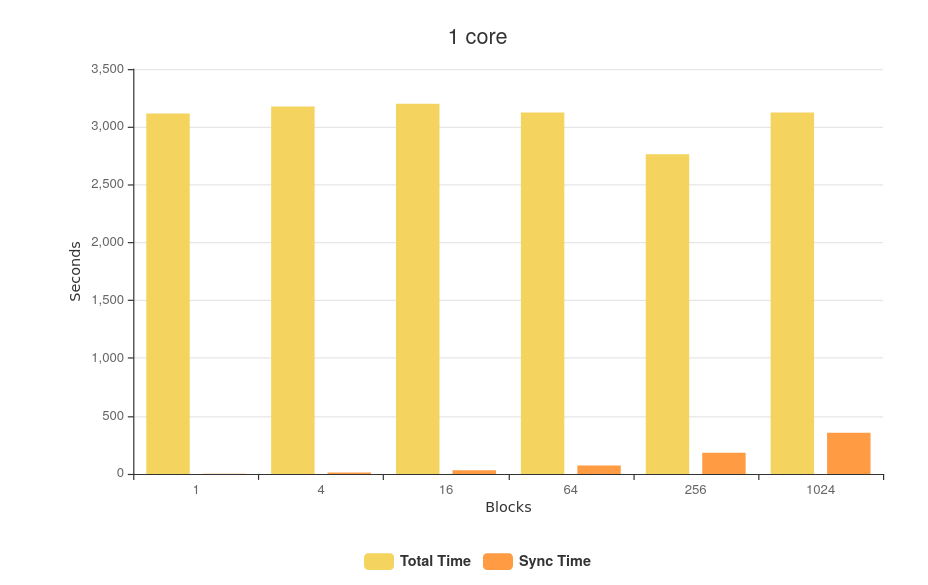
\includegraphics[width=0.6\linewidth, height=180pt]{block_result.png}
    \caption{Тестирование блочного подхода на одном ядре. По вертикальной оси - время в секундах: желтым цветом - общее время работы модели; оранжевым - время на синхронизации блоков. По горизонтальной оси - количество блоков в разбиении.}
    \label{fig:block_res}
\end{figure}
    
Был протестирован блочный подход на одном ядре CPU, т.е. последовательная версия модели.
Расчет проводился на сетке с размером 1525 x 1115 точек.
%Тестирование проводилось на процессоре Intel Xeon Silver 4214.
На рис. \ref{fig:block_res} показано время работы модели в зависимости от количества блоков, участвующих в разбиении области. Видно, что с увлечением количества блоков в разбиении (т.е. с уменьшением размера блока т.к. разбиение на блоки равномерное) общее время расчета модели увеличивается из-за затрат на копирование границ блоков на внерасчетные границы соседних блоков.
Когда размеры блоков становятся достаточно малыми, а именно когда разбиение начинает состоять из 256 блоков, происходит ускорение на 12\% по сравнению с неблочным подходом за счет эффективной работы с кэш памятью в блочном подходе.
И хоть общее время расчета продолжает далее увеличиваться с уменьшением размера блоков, при 1024 блоков в разбиении оно выравнивается со временем неблочного подхода.
Из всего этого можно сделать вывод, что, если выбирать малые размеры блоков, то эффективная работа с кэш памятью компенсирует затраты на копирование границ блоков при синхронизации.
Для рассмотренной акватории получилось, что оптимальный размер блока, получаемый
при разбиении области на 256 блоков, соответствует размеру 95 на 69 точек. Поскольку в вычислениях используются числа с плавающей запятой двойной точности (64 бита на одно число), то один такой блок занимает около 50 Кбайт в памяти.

\begin{figure}[!ht]
	\begin{minipage}{0.5\linewidth}
	\centering
	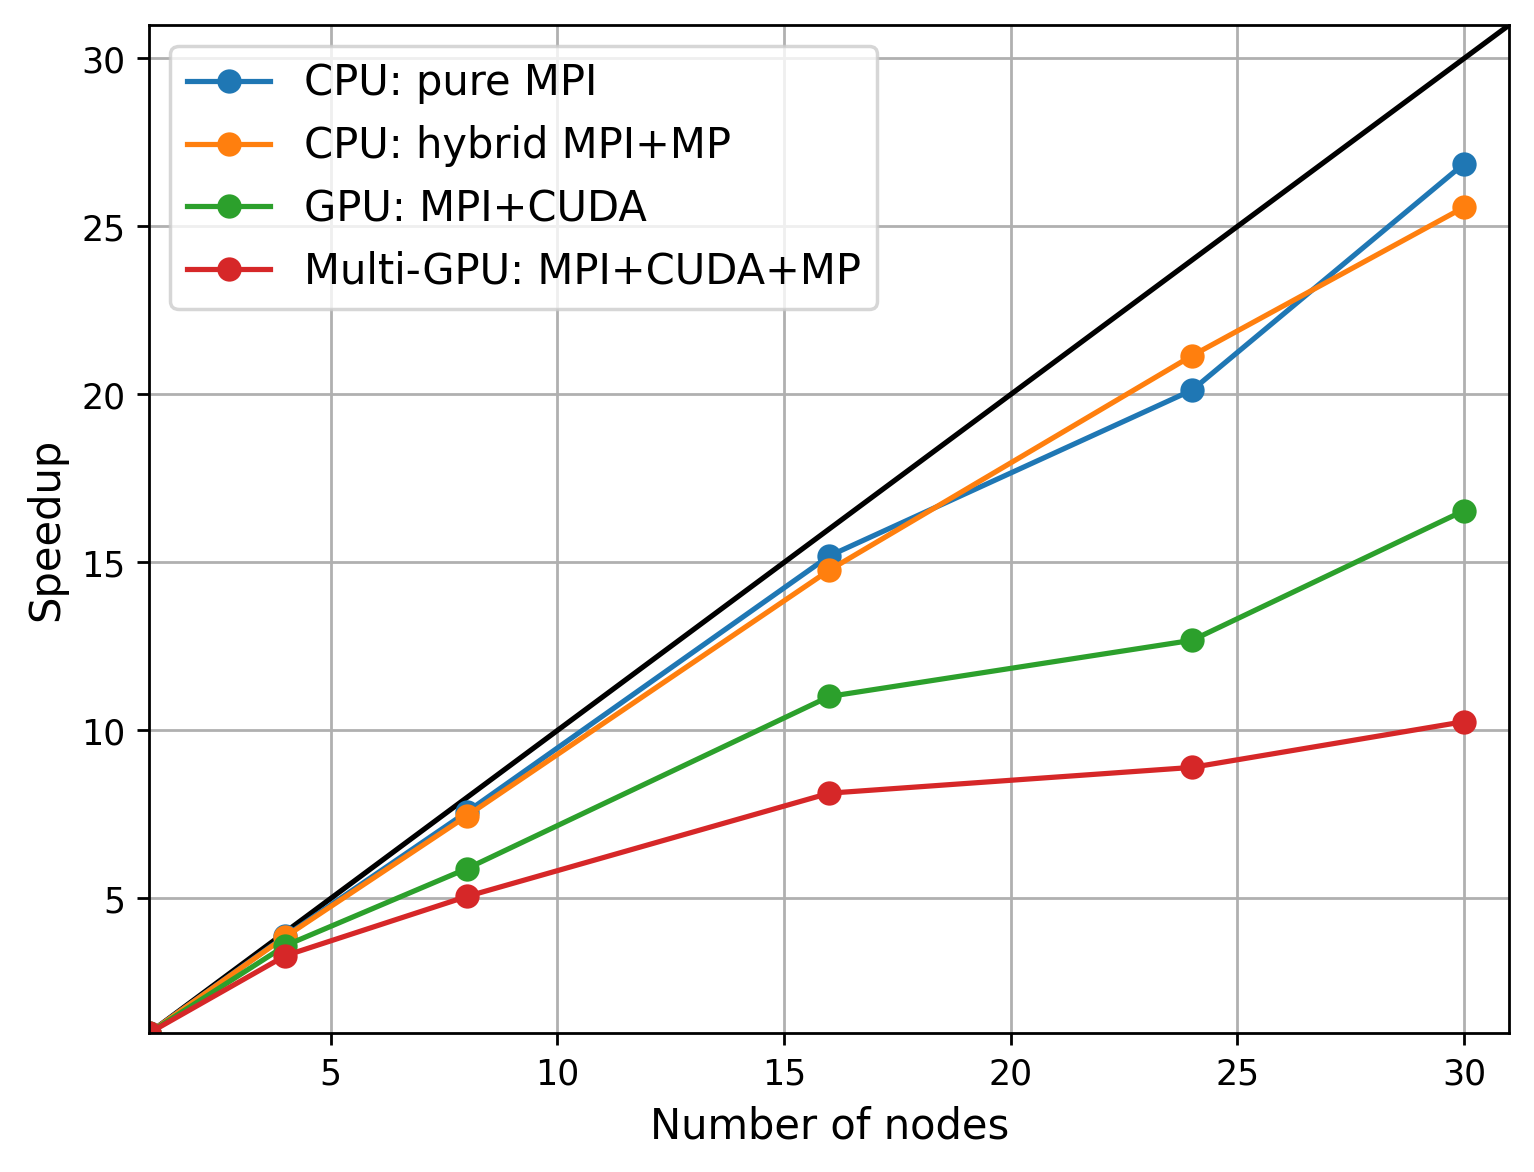
\includegraphics[width=\linewidth]{v3_3_6100x4460_pascal_speedup_multiGPU_V.png}
	\subcaption{Ускорение}
	\end{minipage}
	\begin{minipage}{0.5\linewidth}
	\centering
    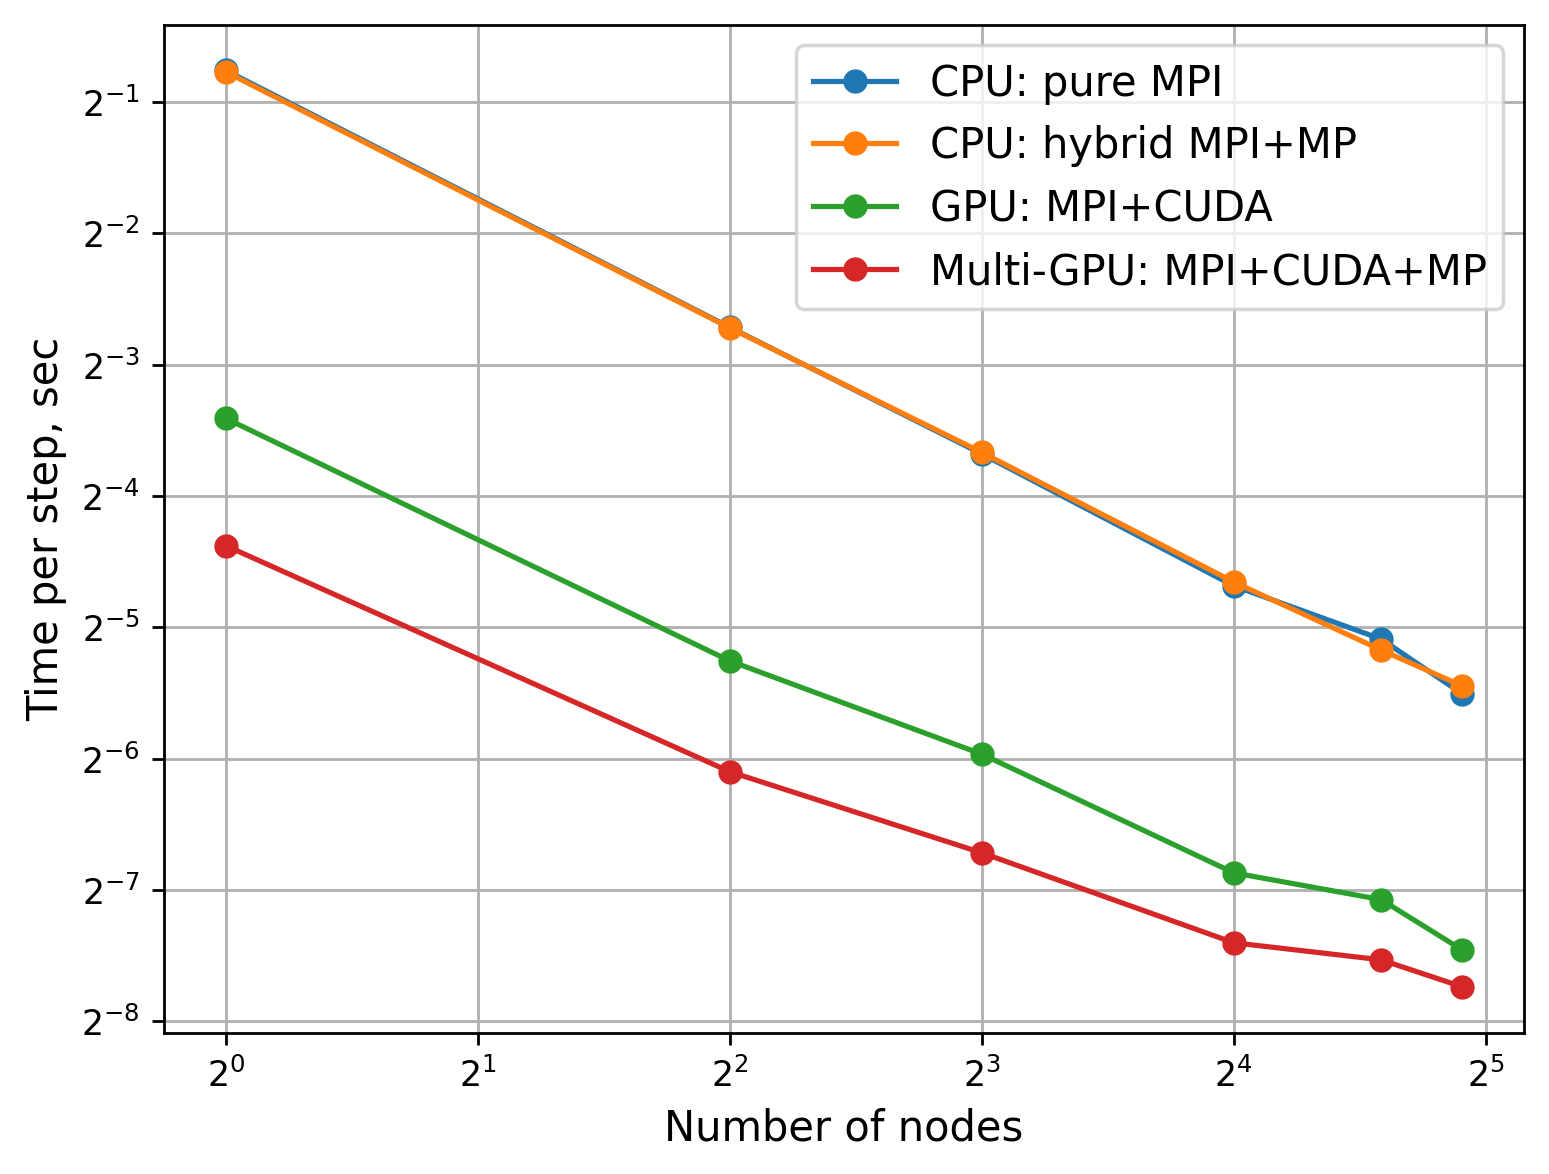
\includegraphics[width=\linewidth]{v3_3_6100x4460_pascal_time_multiGPU_V.png}
	\subcaption{Время одного шага модели (в логарифмической шкале)}
	\end{minipage}
	\vspace{3pt}
	\caption{Масштабирование производительности на разделе Pascal для размера сетки 6100 $\times$ 4460.}
	\label{fig:TheBox}
\end{figure}

Был проведён анализ эффективности и масштабируемости гибридных методов для расчётов мелкой воды с использованием GPU в сравнении с методами расчётов на CPU при размере сетки 6100 x 4460 точек (см. рис \ref{fig:TheBox}).
Представленные результаты на рисунке получены с использованием 30 узлов раздела Pascal суперкомпьютера Ломоносов-2. Чистый MPI подход и гибридные MPI-OpenMP подходы на CPU демонстрируют близкое к линейному (черная линия на рисунке) масштабирование до 30 узлов (всего 360 ядер).
Однако гибридный подход MPI-OpenMP не смог превзойти чистый MPI подход на этом суперкомпьютере. 
Шаблон MPI-OpenMP-CUDA с использованием нескольких GPU на вычислительном узле позволяет выполнять вычисления на 60 GPU с использованием 30 узлов и демонстрирует лучшую производительность благодаря эффективному использованию всех вычислительных ресурсов на узле.
Этот подход имеет в два раза лучшую производительность до 16 узлов, чем шаблон MPI-CUDA с одним GPU на узел, но затем разница в производительности уменьшается из-за небольшого размера подобласти на графический процессор.
Расчет на одном GPU превосходит любой шаблон вычислений на CPU примерно в 6.3 раза, как видно из графиков. 
Несмотря на то что масштабирование производительности на GPU хуже, чем на CPU, вычисления на GPU по-прежнему превосходят вычисления на CPU в 4.7 раза при использовании 60 GPU и 360 ядер CPU на 30 узлах.

\begin{figure}[!ht]
	\begin{minipage}{1\linewidth}
	\centering
	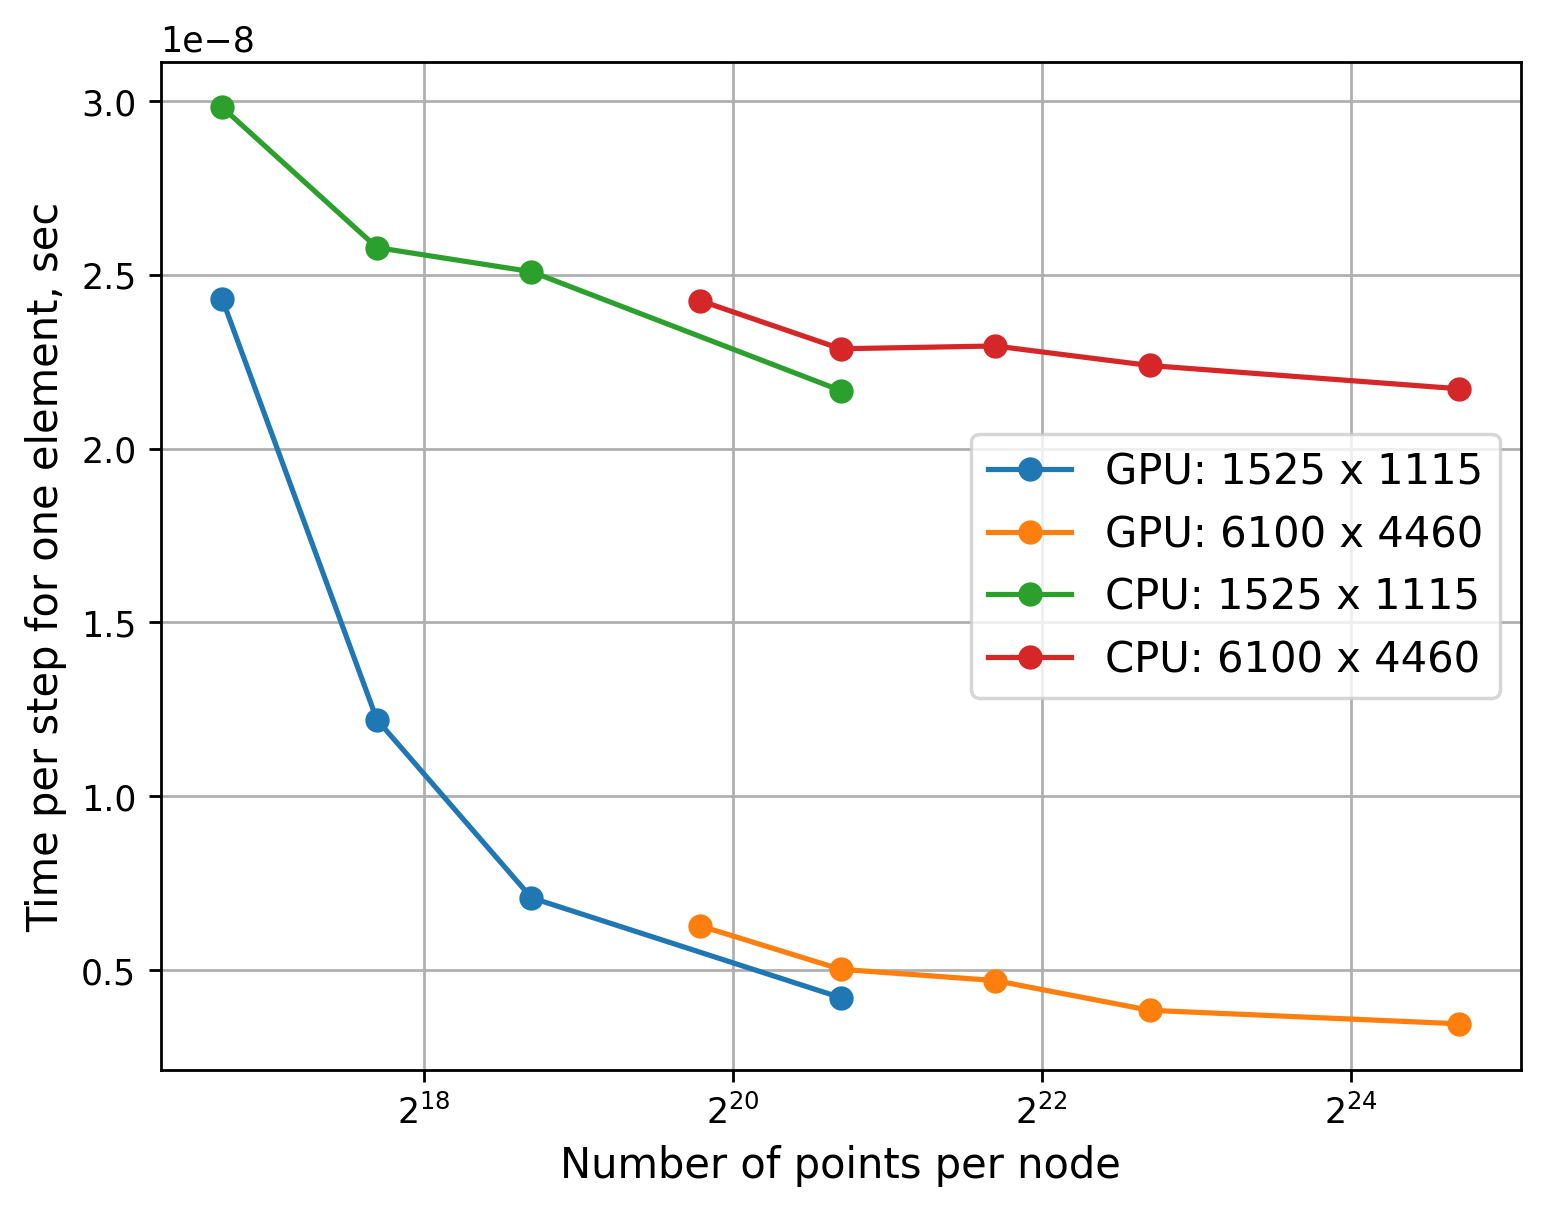
\includegraphics[width=0.5\linewidth]{v3_3_pascal_analysic_fix_1.png}
	\end{minipage}
	\vspace{3pt}
	\caption{Время на одну точку в вычислительной сетке (в логарифмической шкале). Был использован раздел Pascal суперкомпьютера Ломоносов-2.}
	\label{fig:TheBox_full}
\end{figure}

Мы также провели сравнение масштабирования производительности на CPU и GPU при размере сетки 1525 x 1115.
На рисунке \ref{fig:TheBox_full} показано время на одну точку в вычислительной сетке для расчетов на CPU и GPU с размерами сеток 1525 x 1115 и 6100 x 4460.
Из графика видно, что производительность на одну точку сетки на GPU резко снижается после $2^{19}$ точек на узел, в то время как производительность на CPU хорошо масштабируется до $2^{17}$ точек на узел. 
Следовательно, можно заключить, что GPU значительно чувствительнее к размеру сетки, в сравнении с CPU.
Это обусловлено двумя основными факторами.
Во-первых, накладные расходы на коммуникации, включая передачу данных между CPU и GPU, могут превысить время вычислений и стать узким местом производительности на GPU.
Во-вторых, небольшие подобласти приводят к более эффективному использованию кеш-памяти при вычислениях только на CPU, но не могут насытить вычисления и полностью скрыть задержки памяти на GPU.

Чтобы дополнительно исследовать масштабирование производительности на GPU, мы протестировали асинхронный шаблон вычисления MPI-OpenMP-CUDA, который перекрывает передачу данных с выполнением ядра по времени на GPU. Эксперименты на сетке размером 6100 × 4460 проводились на разделе Volta суперкомпьютера, включая Nvidia Tesla V100 на узлах.
На рисунке \ref{fig:asyncGPU_onenode} продемонстрированы показатели производительности при использовании разного числа блоков в блочной подходе на одном GPU. Видно, что асинхронный шаблон вычислений на GPU превосходит синхронный шаблон вычислений на 17\% благодаря параллельному выполнению ядра и передаче данных.
На рисунке \ref{fig:asyncGPU_onenode} показано производительность при использовании различного числа блоков в блочном подходе на одном GPU. Мы видим, что асинхронный шаблон вычислений на GPU превосходит синхронный на 17\% из-за перекрывания выполнения ядра и передачи данных по времени.
Рисунок \ref{fig:asyncGPU} показывает масштабирование производительности асинхронного шаблона вычислений на GPU при оптимальном числе блоков (8 блоков на GPU, как показано на рисунке \ref{fig:asyncGPU_onenode}) по сравнению с синхронным шаблоном вычислений на графических процессорах.
Этот эксперимент показывает, что асинхронный шаблон лучше масштабируется до 8 узлов и на 28\% быстрее на 8 графических процессорах по сравнению с синхронным шаблоном вычислений.
Кроме того, данный эксперимент показывает, что перекрывание выполнение ядра с передачей данных по времени на GPU компенсирует накладные расходы на копирование граничных значений блоков во время синхронизации в блочном подходе.
Однако это утверждение справедливо только для достаточно больших вычислительных областей.

\begin{figure}[!ht]
	\begin{minipage}{1\linewidth}
	\centering
	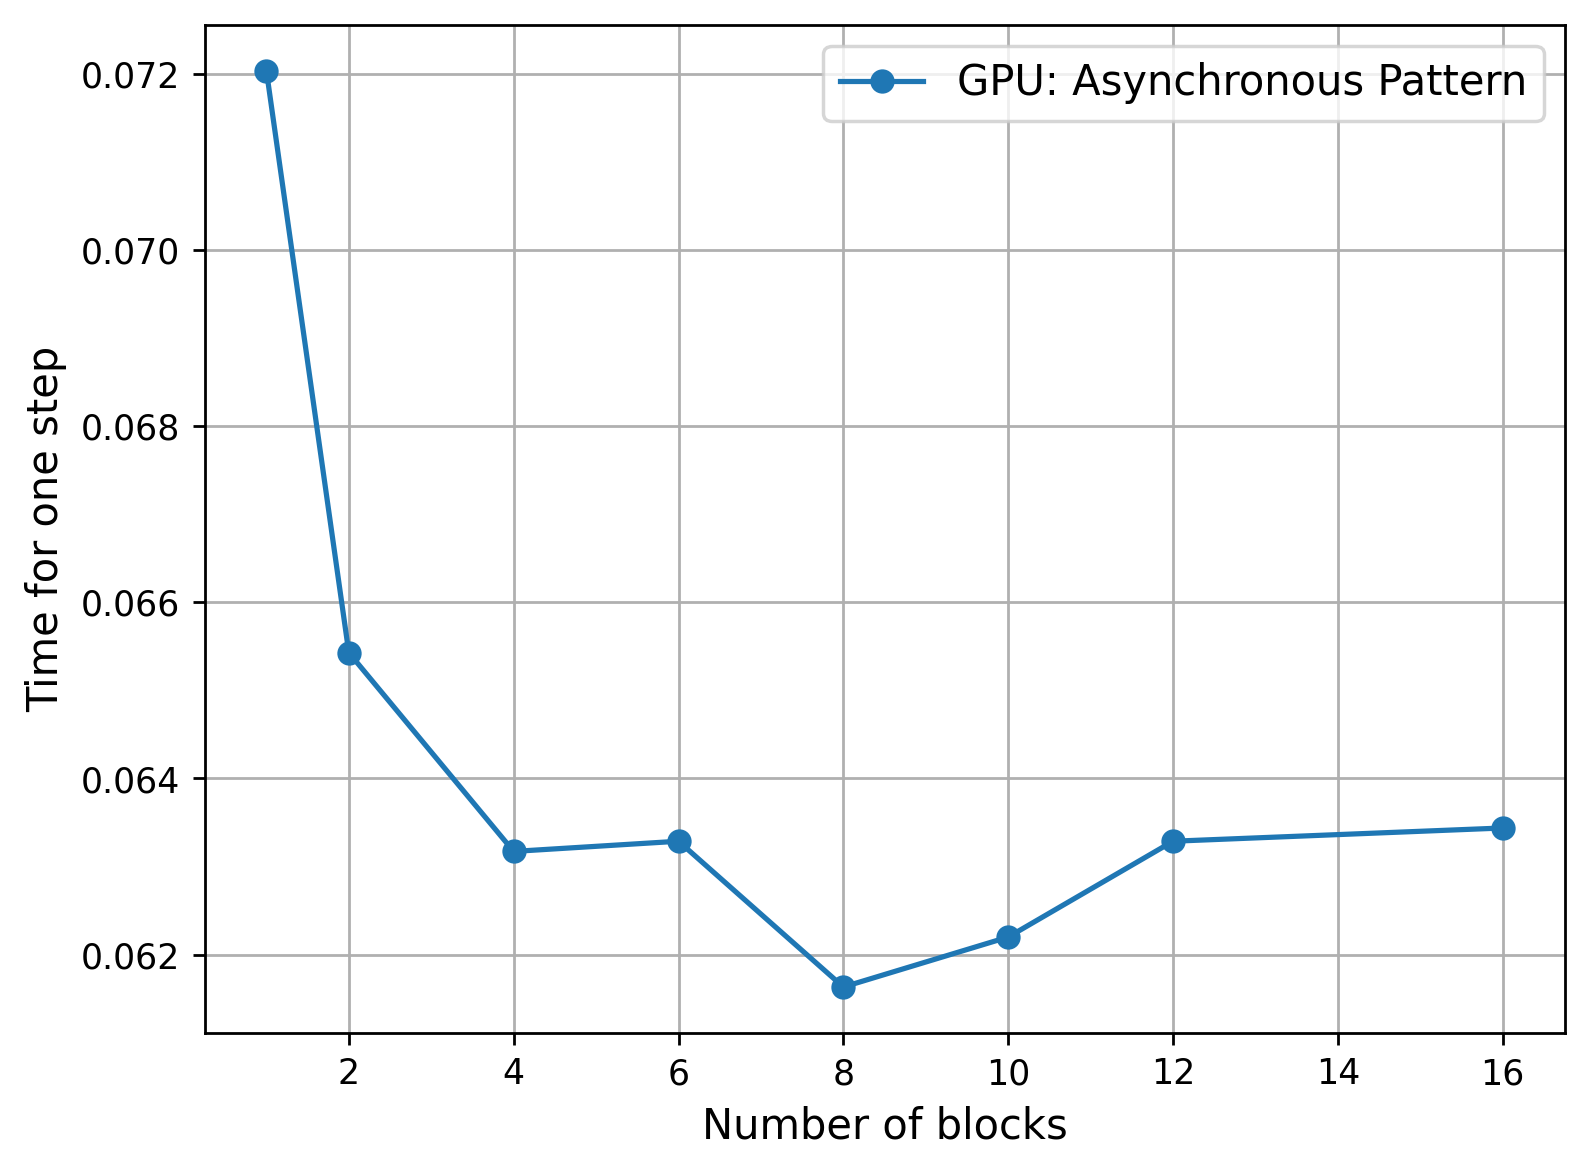
\includegraphics[width=0.5\linewidth]{v3_3_6100x4460_volta_async_blocks.png}
	\end{minipage}
	\vspace{3pt}
	\caption{Время на один шаг модели (в логарифмической шкале) на одном GPU V100 для сетки размером 6100 $\times$ 4460.}
	\label{fig:asyncGPU_onenode}
\end{figure}

\begin{figure}[!ht]
	\begin{minipage}{0.5\linewidth}
	\centering
	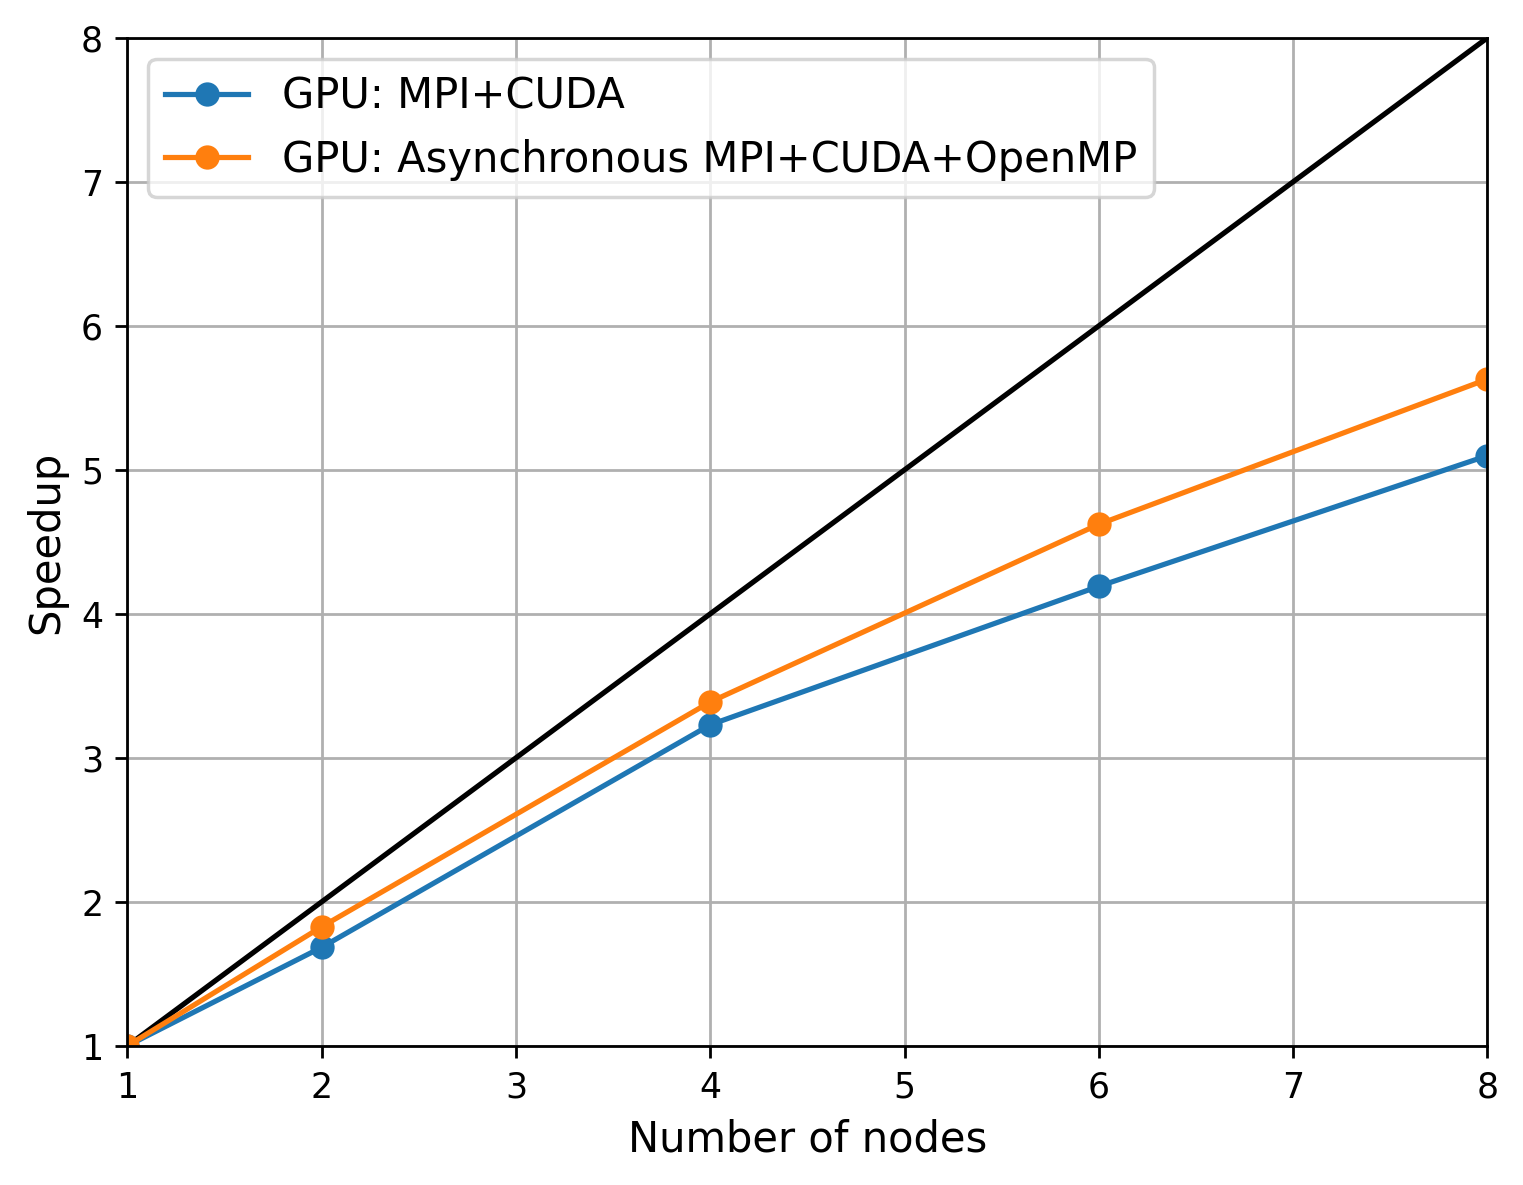
\includegraphics[width=1\linewidth]{v3_3_volta_speedup_renamed.png}
	\subcaption{Ускорение}
	\end{minipage}
	\begin{minipage}{0.5\linewidth}
	\centering
	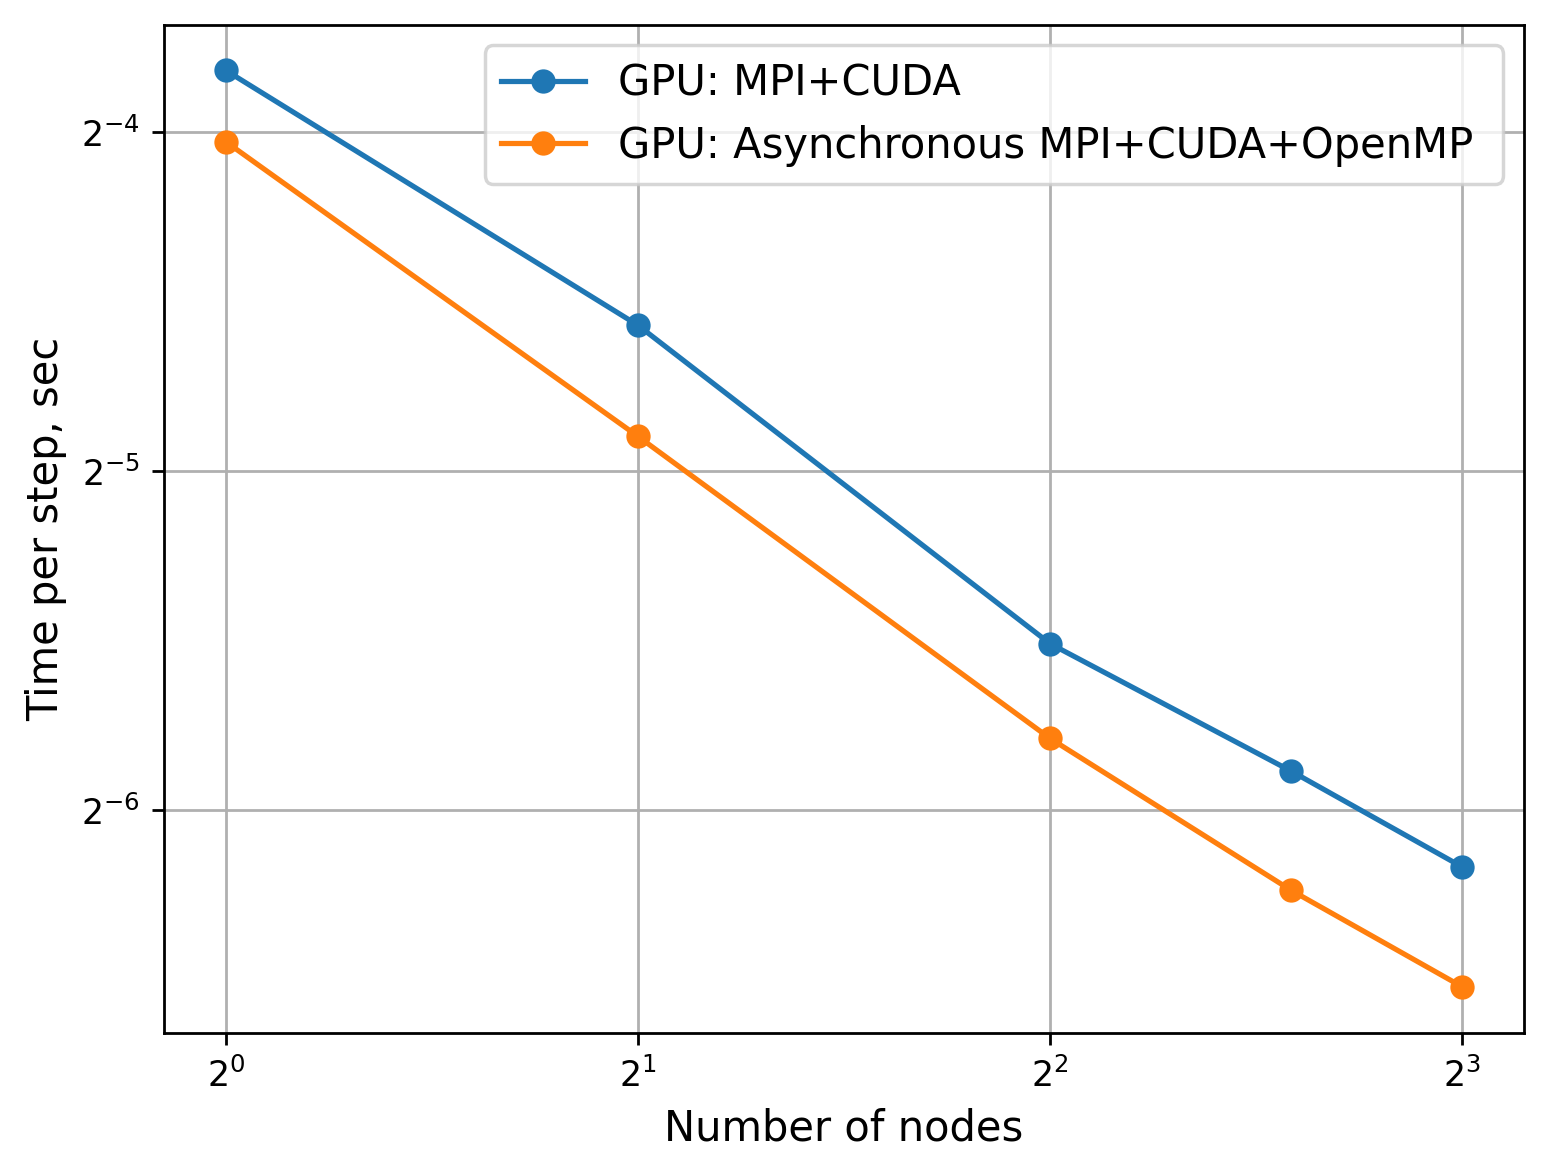
\includegraphics[width=1\linewidth]{v3_3_volta_time_renamed.png}
	\subcaption{Время на один шаг модели (в логарифмической шкале)}
	\end{minipage}
	\vspace{3pt}
	\caption{Масштабирование производительности на GPU V100 для размера сетки 6100 $\times$ 4460.}
	\label{fig:asyncGPU}
\end{figure}

\section{Тестирование Азовского Моря}\label{sec:ch3/sec1}

Азовское море представляет собой подходящий регион для тестирования двумерных численных моделей мелкой воды, так как его гидродинамические процессы могут быть точно и эффективно описаны такими моделями в связи с его относительной мелководностью \cite{Azov}.
Кроме того, вычислительная область Азовского моря обладает значительным количеством наземных точек, что делает целесообразным применение техники балансировки загрузки.
На рисунке \ref{fig:LB} показано, что более половины блоков полностью находятся на суше при делении области на блоки небольшого размера.
Вторая серия экспериментов была проведена в Азовском море с целью оценить масштабирование производительности модели мелкой воды с неравномерной нагрузкой на процессоры и продемонстрировать преимущества использования метода балансировки нагрузки для вычислений на CPU и GPU.
Мы провели тестирование моделей с разным пространственным разрешением: 250 метров (сетка размером 1525 $\times$ 1115) и 62.5 метров (сетка размером 6088 $\times$ 4448). Моделирование было проведено в течение одних суток модельного времени, с общим числом шагов 86400.  

%Метрика $LB$ отвечает за балансировку разделения в терминах нагрузки на процессоры и определяется следующим образом. Предположим, что разделение происходит на $k$ поддоменов для $p$ процессоров, тогда $LB$ определяется как уравнение 5, где $\max_{1 \leq i \leq k} W_i$ - это максимальная нагрузка $i$-го поддомена, а $\sum_{i=1}^k W_i$ - это общая нагрузка всей вычислительной области.

Расчет нагрузки выполняется по-разному для вычислений на CPU и GPU.
Для CPU метрика загруженности подобласти представляет собой сумму "влажных" точек в подобласти, как было показано в разделе \ref{sec:ch2/sec3/lb}, см. уравнение \ref{eq:LB}.
Однако для графических процессоров нагрузка подобласти представляет сумму всех точек (как "сухих", так и "влажных").
Из-за расходящихся путей выполнения, производительность на GPU не уменьшается с увеличением доли "влажных" точек, в отличие от CPU \cite{kirk10}.
Поэтому для вычислений на GPU мы равномерно распределяем блоки из блочного разбиения между GPU, исключая полностью блоки, которые попадают на сушу.

Как упоминалось ранее, блочное разбиение разделяет область на небольшие блоки и распределяет их среди доступных процессоров.
С одной стороны, использование небольшого числа блоков в разделении приводит к высокому значению метрики $LB$ (см. уравнение \ref{eq:LB}) и несбалансированным подобластям процессоров.
С другой стороны, использование большого числа блоков в разделении приводит к высоким накладным расходам при копировании граничных значений блоков во время синхронизации процессоров, что особенно важно для вычислений на GPU, поскольку мы должны передавать данные между CPU и GPU для каждого блока.
Поэтому количество блоков $k$ в разделении выбирается адаптивно для распределения среди $p$ процессоров в соответствии с следующим критерием:

\begin{equation} \label{eq:LB_GPU} 
k(p) = \min_{n=0,1,...} \{ 4^n ~|~ LB(4^{n}, p) - LB(4^{n+1}, p) < 0.15 \}
\end{equation}


\begin{table} [htbp]
\centering
%\begin{threeparttable}% выравнивание подписи по границам таблицы
\caption{Метрики LB для Азовского моря с разрешением 250 метров}\label{tab:CPULB}
	\begin{tabular}{cccc}
	$p$ & $LB$ для 256 блоков & $LB$ для 1024 блоков & $LB$ для 4096 блоков \\
    \hline
	48    &  1.371   &  \textbf{1.045}  &  1.012 \\
    96    &  1.802   &  \textbf{1.154}  &  1.022 \\
	192   &    -     &  1.385  &  \textbf{1.070} \\
	\hline
	\end{tabular}
%\end{threeparttable}
\end{table}

Таблица \ref{tab:CPULB} демонстрирует оптимальное количество блоков для вычислений на разном количестве процессоров согласно описанному критерию; оптимальное количество блоков выделено в таблице.

Мы провели тестирование модели Азовского моря на разделе Pascal суперкомпьютера Ломоносов-2.
На рисунке \ref{fig:AzovSea} показана зависимость производительности модели с балансировкой нагрузки по сравнению с моделью без балансировки нагрузки на CPU при размере сетки 1525 $\times$ 1115 и на GPU при размере сетки 6088 $\times$ 4448.
Мы рассматривали только чистый MPI подход на CPU и сравнивали асинхронный шаблон вычислений MPI-OpenMP-CUDA с синхронным шаблоном вычислений MPI-CUDA на GPU.
На одном узле модель вычислялась без балансировки нагрузки.
Мы использовали оптимальное количество блоков в соответствии с критерием \ref{eq:LB_GPU}.
Для проведения вычислений на CPU, было выбрано оптимальное количество блоков в разбиении согласно Таблице \ref{tab:CPULB}; для проведения вычислений на GPU использовались 64 блока для 4 узлов и 256 блоков для 16 узлов.

Как видно из Рисунка \ref{fig:AzovSea}, метод балансирования нагрузки оказывает значительное влияние на производительность модели на CPU – схема с балансированием нагрузки демонстрирует рост на 30\% по сравнению со схемой без балансирования при использовании 16 узлов, при этом демонстрируя сверхлинейное масштабирование благодаря эффективности кэш-памяти за счет использования блоков малого размера.
При работе на GPU можно отметить, что асинхронный подход с балансировкой нагрузки увеличивает производительность на 30\% и 18\% соответственно по сравнению с синхронным и асинхронным шаблонами вычислений без балансирования нагрузки при использовании 16 узлов.
Однако, несмотря на увеличенное разрешение сетки, производительность на GPU масштабируется хуже по сравнению с CPU. Как было отмечено ранее, GPU более чувствительны к размерам задачи по сравнению с CPU (см. рис. \ref{fig:TheBox_full}).
Это особенно важно в данном контексте, поскольку с увеличением числа узлов число точек на GPU значительно снижается из-за наличия наземных точек в вычислительной области.

\begin{figure}[!ht]
	\begin{minipage}{0.5\linewidth}
	\centering
	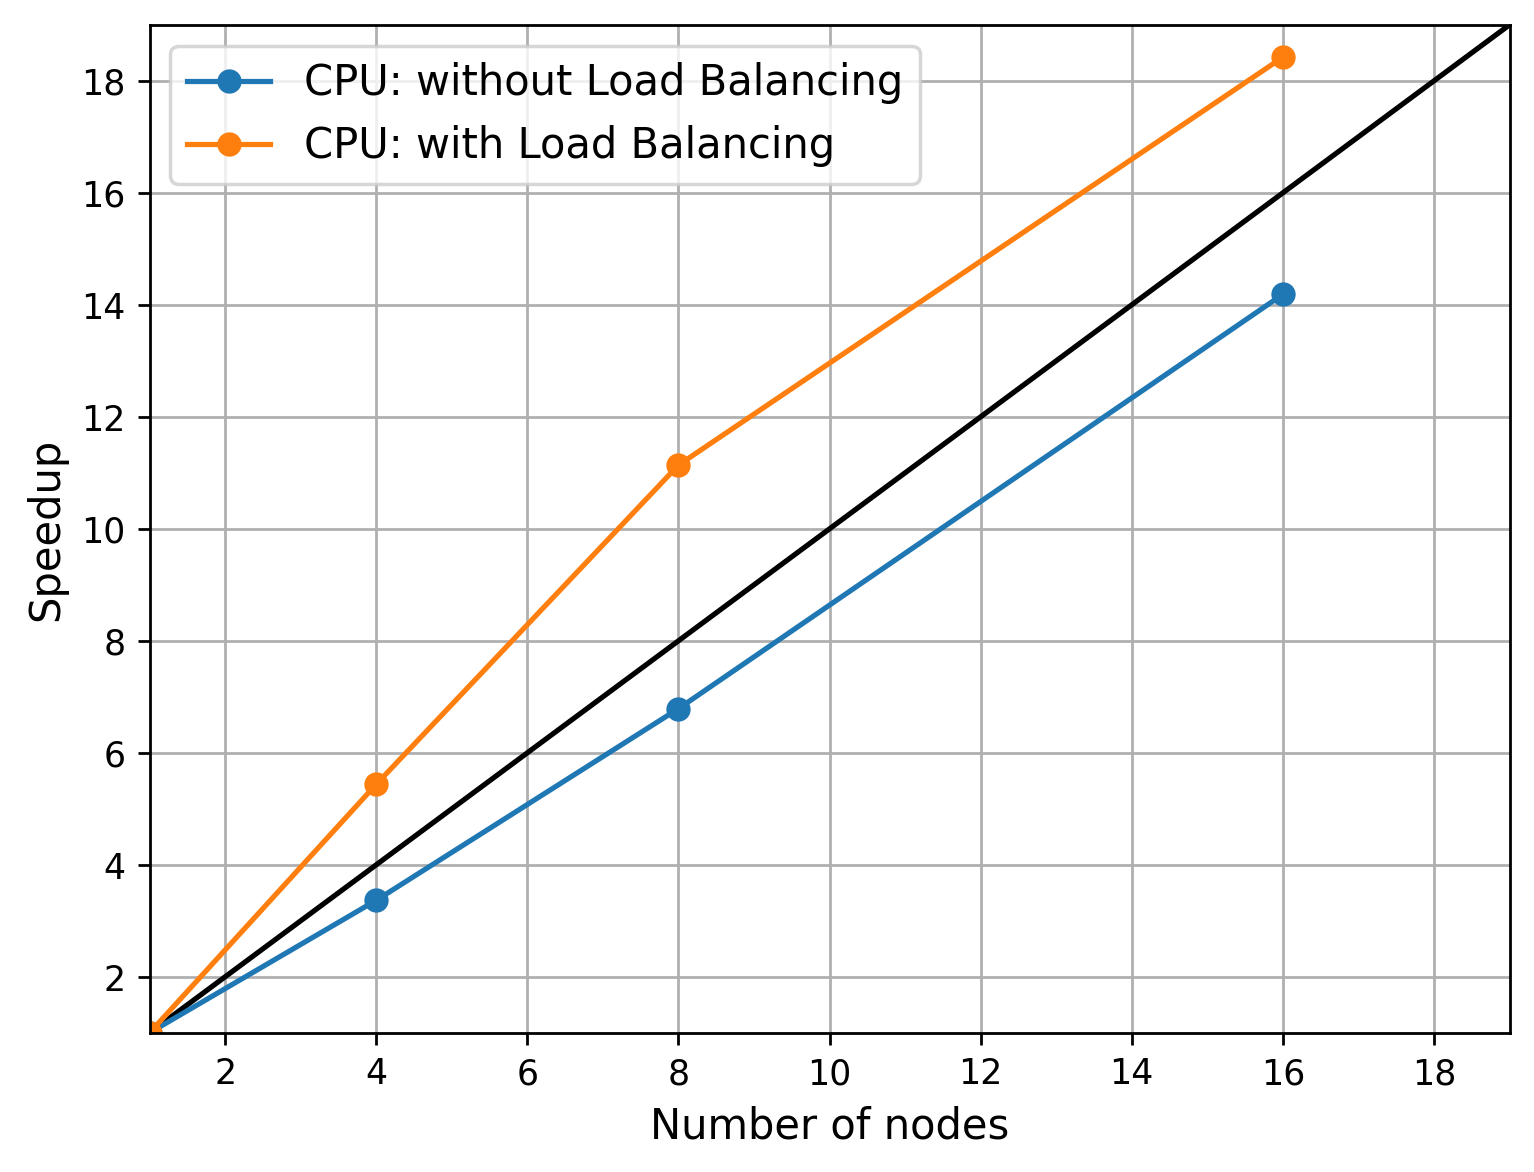
\includegraphics[width=\linewidth]{v3_3_AS250m_pascal_CPU_LB_speedup.png}
	\subcaption{Ускорении CPU версии модели с пространственным разрешением 250 м}
	\end{minipage}
	\begin{minipage}{0.5\linewidth}
	\centering
    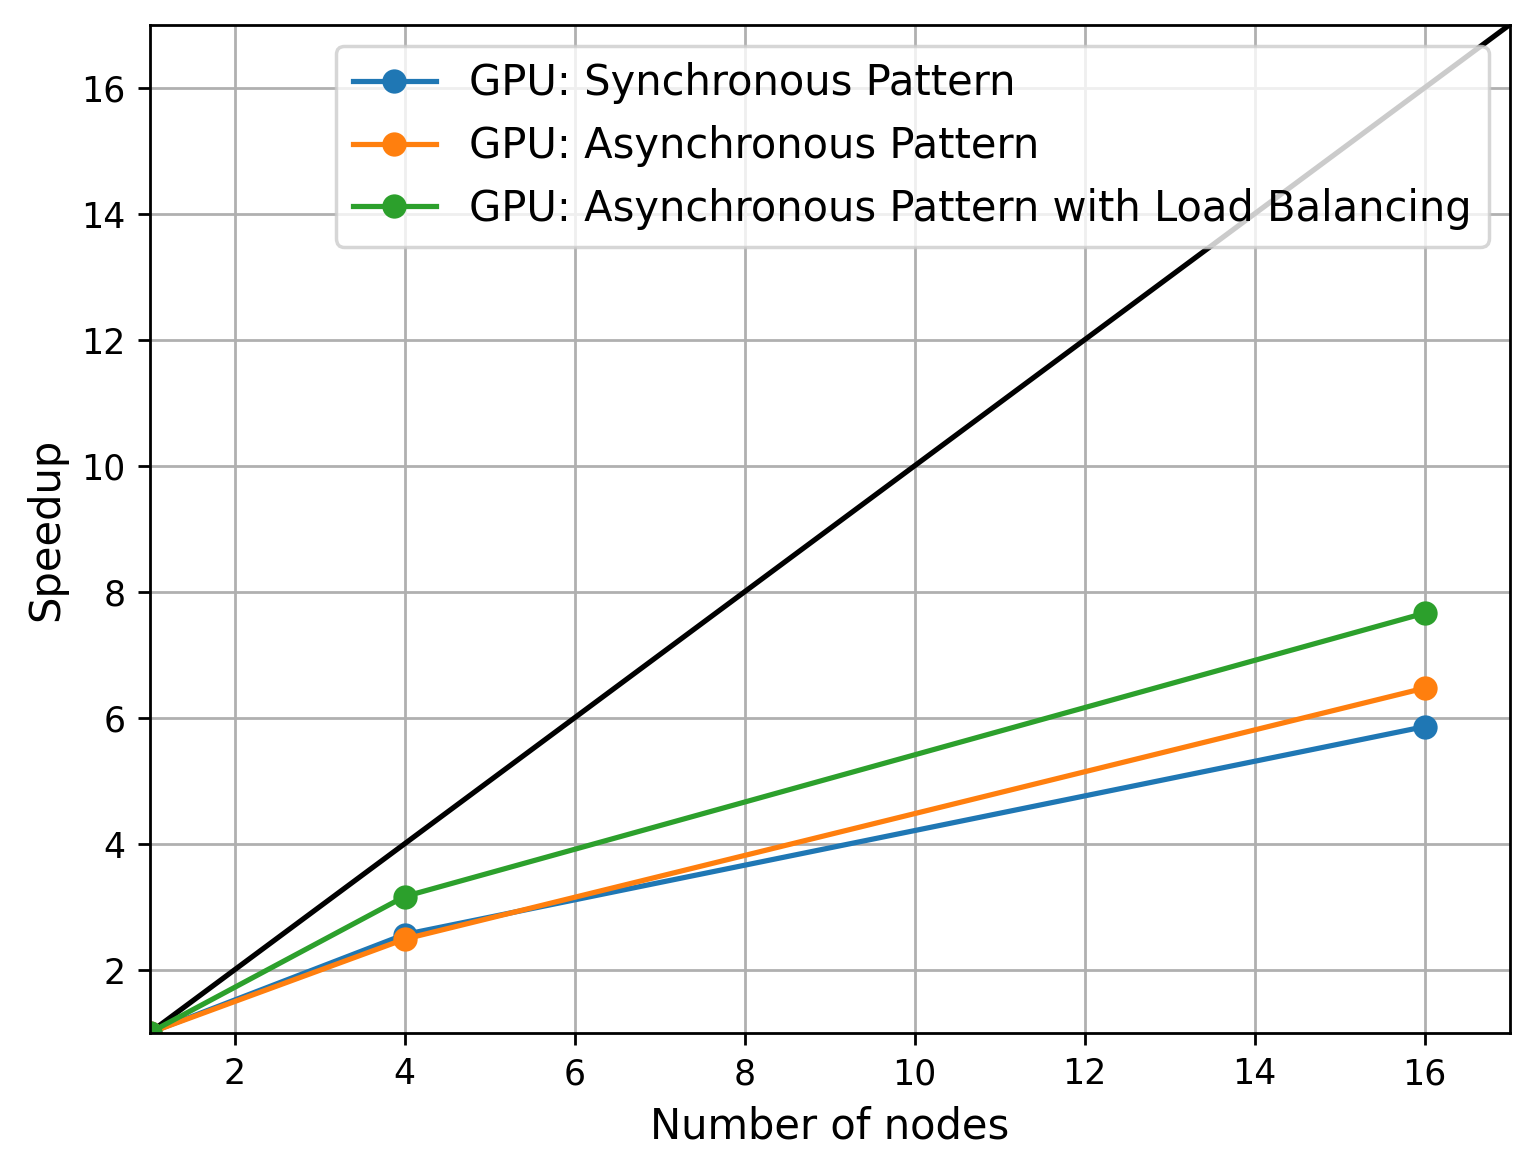
\includegraphics[width=\linewidth]{v3_3_AS62_5m_pascal_GPU_LB_speedup_cut.png}
	\subcaption{Ускорение GPU версии с пространственным разрешением 62.5 метров}
	\end{minipage}
	\vspace{3pt}
	\caption{Масштабирование производительности для акватории Азовского моря. Был использован раздел Pascal суперкомпьютера Ломоносов-2.}
	\label{fig:AzovSea}
\end{figure}

\FloatBarrier
